\chapter{Datenverarbeitung}

Wie bei jeder Anwendung von maschinellen Lernverfahren sind die zugrundeliegenden Daten von äußerster Wichtigkeit.
Im Rahmen dieser Masterarbeit wurden zweierlei Sorten von Daten benutzt:
Einmal wurden am \textit{TableSort} Schüttgutsortierer des Fraunhofer IOSBs Aufnahmen gemacht, 
die dann über mehrere Arbeitsschritte in das richtige Format übersetzt werden.
Zudem existieren der DEM Datensatz \todo{mehr details - was tut der überhaupt}



\section{Datenformatierung}

Zu beginn des Datenverarbeitungskapitel erstmal definieren wie unsere Feature-Label Paare aussehen.
Features eigentlich immer gleich:
die Positionen der letzten \(n\) Zeitschritte (FeatureSize Hyperparameter)
also ein \(2n\) Tupel, mit jeweils \(n\) X-Koordinaten und \(n\) Y-Koordinaten


Labels: Unterscheidung nach Anwendung:

NextStep: Label ist 2-Tupel, X und Y Koordinate
Separator: 
	gegeben ist eine Stelle entlang der Bewegungsrichtung der Teilchen an der der Separator angebracht ist.
	erstes element des Label ist die Koordinate entlang der orthogonalen Achse zur Bewegungsrichtung wo das Teilchen den Separator passiert
	zweites Element ist die Anzahl von Zeitschritten , die das Teilchen noch bis zum Separator braucht.

Important Point: Labels wurden normalisiert und Standardisiert ( \(\frac{TrueVal - Mean}{Standard Diviation}\)
um auszugleichen, dass sich Position und Zeitschritte auf unterschiedlichen Skalen bewegen und dementsprechend unterschiedlich hohe gradienten haben.


Es ist implementiert, dass die verschiedenen Dimensionen unterschiedlich stark gewichtet werden können - Je nach Schüttgut/präzision des Separators
Aber für die evaluierung ist keine Gewichtung vorgenommen worden.

potenziell: Histogramme über die Daten (mehr Teilchen in der Mitte bei Location...)



\section{Eigene Aufnahmen}

\subsection{Versuchsaufbau}

[Beschreibung von der Bonito Kamera, stats usw.]
Zur Aufnahme der Daten wurde eine Bonito CL-400 200 FPS Kamera benutzt, die in Abbildung \ref{pictureCam} zu sehen ist.
Die ist, wie in Abbildung \ref{pictureCam} oberhalb des Förderbandes angebracht.
Die Bilder, die von der Kamera aufgenommen werden, haben eine Auflösung von 2320x1726 Pixeln.

\begin{figure}
    \centering
    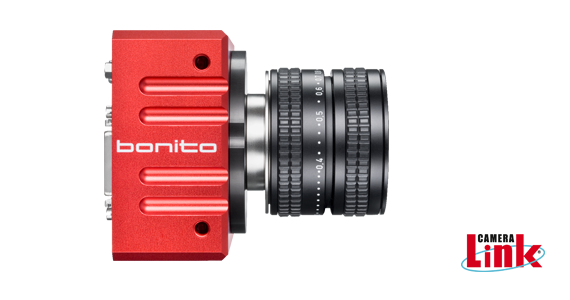
\includegraphics[width=\textwidth]{img/banner-Bonito_cropped}
    \caption{Zur Aufnahme verwendete Kamera [TODO: Quelle Bild]}
    \label{pictureCam}
\end{figure}

\subsection{Schüttgüter-Typen}

Aufgenommen wurden vier verschiedene Schüttgüter, die in Abbildung \ref{schuettgueterSchuessel} zu sehen sind.

\begin{itemize}
    \item Kugeln
    \item grüne Pfefferkörner
    \item Zylinder
    \item Weizenkörner
\end{itemize}

Die Kugeln und der Pfeffer sowie die Zylinder und die Weizenkörner bilden jeweils 
ein Paar aus einem geometrischen Körper und einem echten Objekt, das grob dessen Form ähnelt.

Die Kugeln bestehen aus Holz und haben einen Durchmesser von 5mm.
Die Zylinder bestehen ebenfalls aus Holz. Sie haben eine Länge von 1cm und einen Durchmesser von 3mm.
Die Schüttgüter sind in Abbildung \ref{schuettgueterSchuessel} in Schüsseln 
und in Abbildung \ref{schuettgueterBand} auf dem Förderband zu sehen.
\todo{TODO: Details}

\begin{figure}[h]
	\centering
	\begin{subfigure}[t]{0.4\textwidth}
		\includegraphics[width=\textwidth]{kugel_001_00084_debayer}
		\caption{Kugeln}
	\end{subfigure}
	\quad
	\begin{subfigure}[t]{0.4\textwidth}
		\includegraphics[width=\textwidth]{Pfeffer_003_00020_debayer}
		\caption{Pfeffer}
	\end{subfigure}
	\vskip\baselineskip
	\begin{subfigure}[t]{0.4\textwidth}
		\includegraphics[width=\textwidth]{zylinder_001_00009_debayer}
		\caption{Zylinder}
	\end{subfigure}
	\quad
	\begin{subfigure}[t]{0.4\textwidth}
		\includegraphics[width=\textwidth]{weizen_004_00016_debayer}
		\caption{Weizen}
	\end{subfigure}
	\caption{Verschiedene Schüttgüter}
	\label{schuettgueterSchuessel}
\end{figure}


\section{Datenpipeline}

Die Bilder wurden in Batches von je 3500 gesammelt.
Die Bonito Kamera schreibt sie in Form einer Bayer-Matrix in Bitmap Dateien.
\todo{hier Bayer-Matrix erklären und Bild?}

\begin{figure}
	% \missingfigure{bayer matrix}
	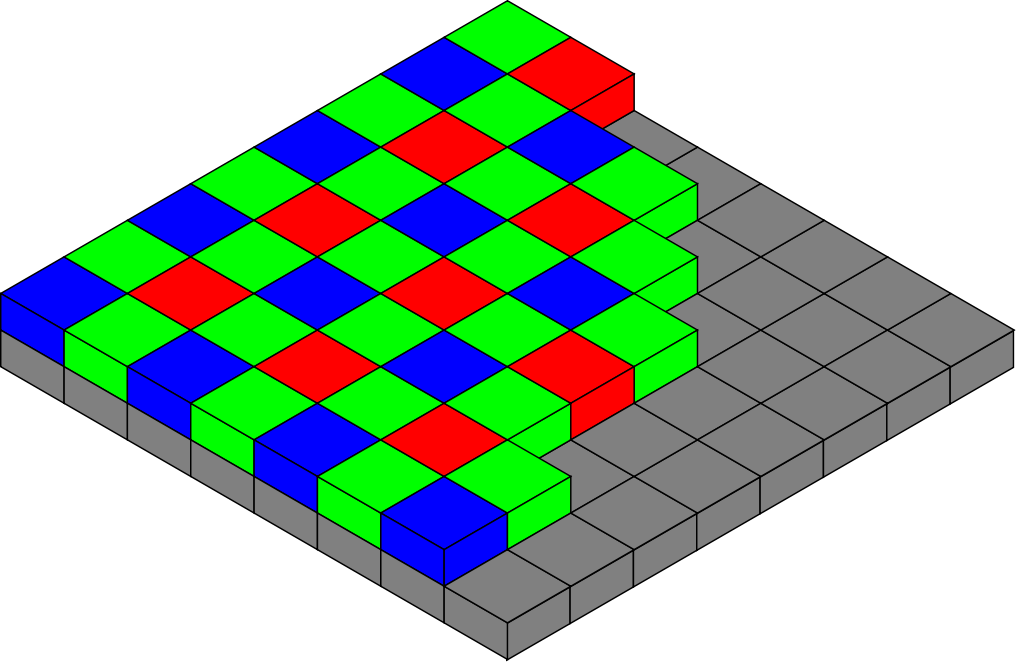
\includegraphics[width=\textwidth]{1024px-Bayer_pattern_on_sensor}
	\caption{Bayer Matrix [TODO: Quelle]}
	% \todo{Quelle Bild!}
	\label{fig:bayerPattern}
\end{figure}

Auf Grund der Menge an Bildern war es sinnvoll die Dateien in das png Dateiformat zu übertragen.
Die Features, die für das Trainieren der Netze benutzt werden, sind die Koordinaten der Mittelpunkte der Objekte.
Um diese zu bestimmten, müssen zunächst die Dateien mittels \textit{demosaicing} rekonstruiert werden um gewöhnliche RGB Bilder zu erhalten.
Die Open Source Computer Vision Library OpenCV hat eine Methode implementiert, die ein Bild von einem Farbraum in einen anderen übertragen kann
und die eingesetzt wurde um die einzelnen Bilder in RGB Farbbilder zu konvertieren.
\todo{Skript ursprünglich von Georg, ein paar changes implementiert bezüglich input und output.}

\begin{figure}[h]
	\centering
	\begin{subfigure}[t]{0.4\textwidth}
		\includegraphics[width=\textwidth]{KugelnCropped}
		\caption{Kugeln}
	\end{subfigure}
	\quad
	\begin{subfigure}[t]{0.4\textwidth}
		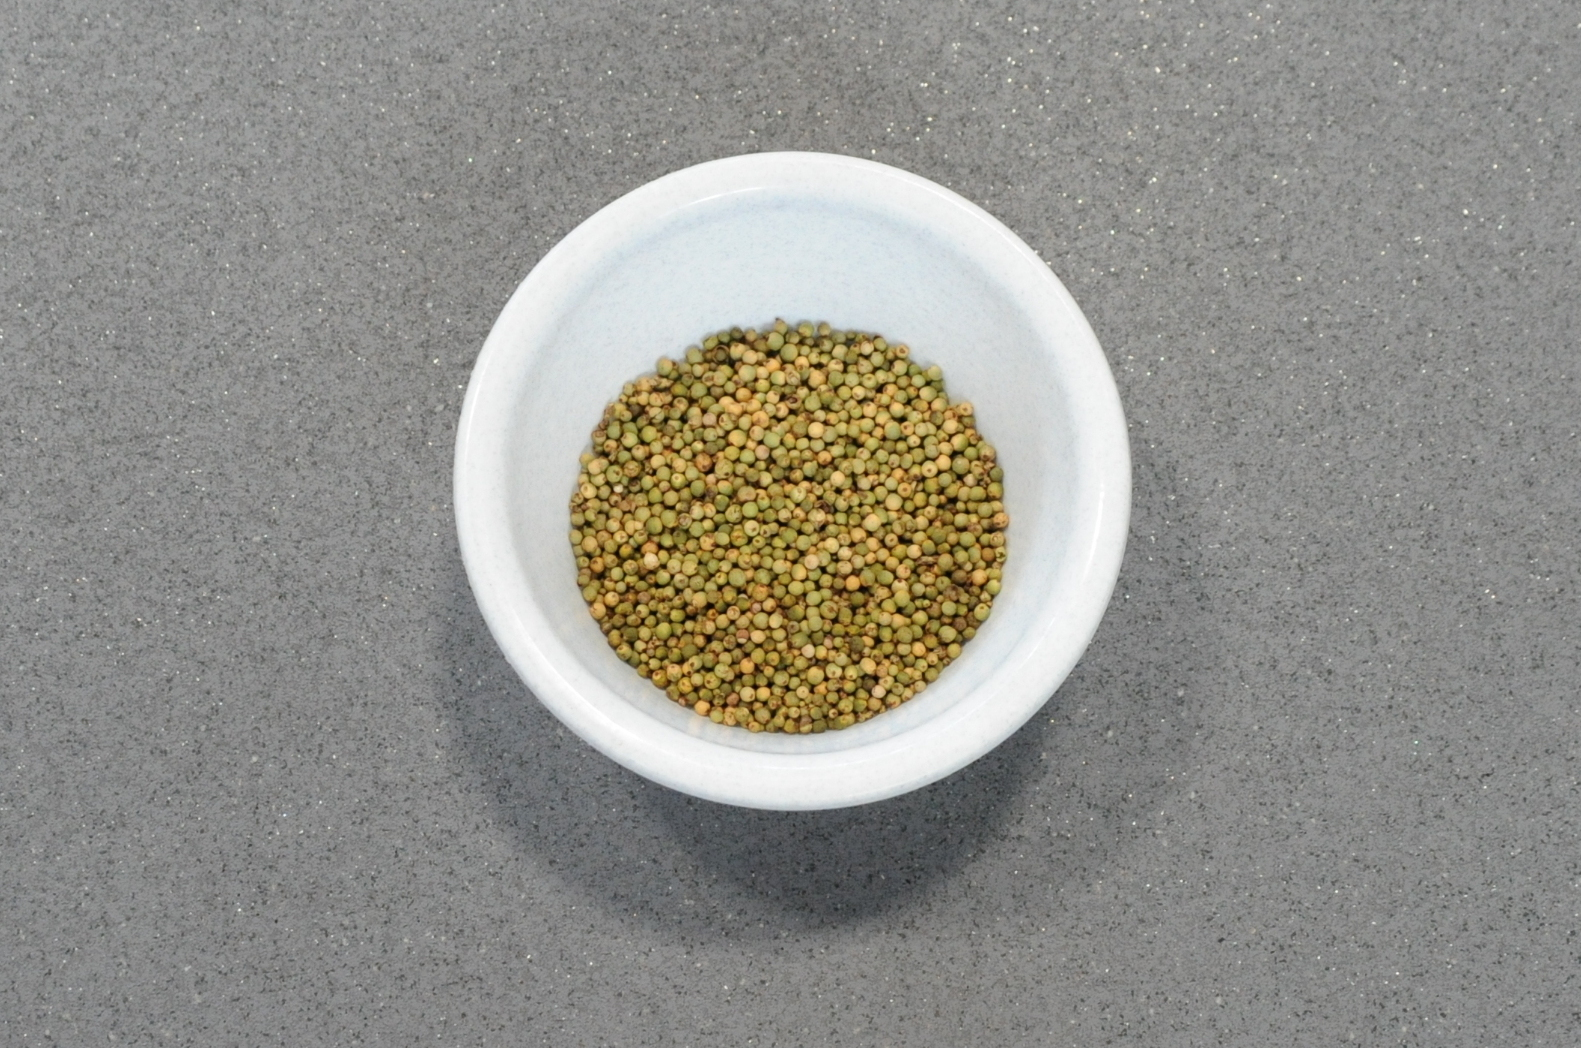
\includegraphics[width=\textwidth]{PfefferCropped}
		\caption{Pfeffer}
	\end{subfigure}
	\vskip\baselineskip
	\begin{subfigure}[t]{0.4\textwidth}
		\includegraphics[width=\textwidth]{ZylinderCropped}
		\caption{Zylinder}
	\end{subfigure}
	\quad
	\begin{subfigure}[t]{0.4\textwidth}
		\includegraphics[width=\textwidth]{WeizenCropped}
		\caption{Weizen}
	\end{subfigure}
	\caption{Verschiedene Schüttgüter auf dem Förderband}
	\label{schuettgueterBand}
\end{figure}


Auf diesen kann dann eine Segmentierung vorgenommen werden.
Hierzu wurde erneut die Computer Vision Library OpenCV benutzt.
\todo{Mehr details: Parameters...}
Das Ergebnis des Segmentierungsscripts [Reference segement.py] ist ein CSV File für jedes Batch.
Eine Zeile repräsentiert ein Bild aus dem Batch, also einen Zeitschritt.
Zu Beginn jeder Zeile steht zunächst die Frame Nummer, gefolgt von der Anzahl der detektierten Partikel
und den X- und Y-Koordinaten der detektierten Partikel.
\todo{TODO: Verifizieren}
Die Mittelpunkte in diesem CSV File werden nun mittels des in MATLAB implementierten TrackSort Algorithmus einzelnen Tracks zugeordnet,
die dann wiederum in einem neuen CSV File gespeichert werden.
Die einzelnen Tracks werden als Spaltenpaare dargestellt mit jeweils einer Spalte für die X- und Y-Koordinaten zu einem jeweiligen Zeitpunkt.
Ein Ausschnitt aus einer solchen Datei ist in Tabelle \ref{tableTracks} zu sehen.


\begin{table}[ht]
\caption{Beispielhafter Ausschnitt aus einem CSV File} 
\begin{adjustbox}{width=1\textwidth}
\begin{tabular}{c|c|c|c|c|c}%
    %\bfseries Person & \bfseries Matr.~No.% specify table head
    
    \bfseries TrackID\_1\_X & \bfseries TrackID\_1\_Y & \bfseries TrackID\_2\_X  & \bfseries TrackID\_2\_Y & \bfseries TrackID\_3\_X & \bfseries TrackID\_3\_Y
    \csvreader[head to column names]{docExample.csv}{}% use head of csv as column names
    {\\\hline\csvcoli&\csvcolii&\csvcoliii&\csvcoliv&\csvcolv&\csvcolvi} % specify your coloumns here
    \end{tabular}
\end{adjustbox}

\label{tableTracks}
\end{table} 


\section{Simulierte Daten}

Die DEM Daten, wo sie herkommen, was der unterschied ist zu den selbstaufgenommenen Daten. Vorteile und Nachteile...

\subsection{Menge}

Insgesamt wurden 177954 Bilder aufgenommen.

Es wurden 
7538 Kugeln in 15 Batches,
7056 Pfefferkörner in 13 Batches,
17049 Zylinder in 11 Batches
und 8549 Weizenkörner in 13 Batches aufgenommen.
\todo{outdated: neue Zählung ist notwending}

\todo{Table mit Anzahl von Elementen in verschiedenen Batches}

\begin{figure}
    \centering
    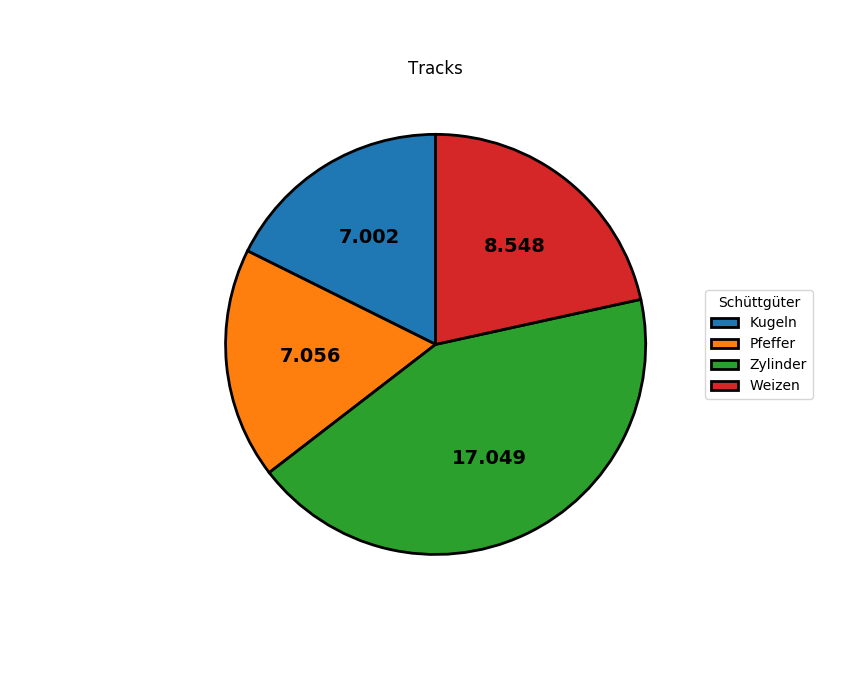
\includegraphics[width=\textwidth]{img/scaledPieChart-trimmed}
    \caption{Verteilung Schüttgut Elemente nach Sorte}
    \label{piechartSchuettgut}
\end{figure}


Menge in gecleanten Daten:

7343 Kugeln
6824 Pfefferkörner
15760 Zylinder
8426 Weizenkörner


\section{Daten Postprocessing}

[FilterTracksByAngle] [FilterByVectorLengthChange]

[Data Augmentation: Spiegeln]

Als Data Augmentation bezeichnet man Verfahren, die das eigene Set an Daten erweitern ohne zusätzliche Daten aufzunehmen
in dem man aus den bestehenden Daten synthetische Daten generiert.
\todo{nur Trainingsset}
Ausreichend viele Datenpunkte zu haben ist notwendig um mit neuronalen Netzen eine gute Performance zu erzielen.
Die synthetischen Beispiele müssen jedoch plausibel sein, da sie sonst die \todo{performance verschlechtern}

~~~

- bei Bildern normalerweise Rotieren, Translation, Ausschnitte...
- Hier: Spiegeln in einem Band - an der Mitte, nicht die Ränder mit nehmen - Kamera nicht perfekt zentriert
- führt zu: Beinah verdoppelung der Feature-Label-paare fürs training.

\section{Trainingsbeispiele}

Train - Test - Validation - Split:
Train - test, 90\% zu 10\%.
Validation nur für die sets auf denen das Hyperparameter Tuning gemacht wurde
[ungefähres ]


Features sind für NextStep und Separator gleich.
(Unclear yet:Separator müssen insgesamt die Trainingsbeispiele gefiltert werden? Zumindest für die Evaluation? TODO!)

Labels:
Sehr straight forward für NextStep (Literally), einfach die nächste Zeile im Track jeweils für X und Y

für separator slightly more complicated: 
Element des Tracks vor und hinter der Separator position (entlang der Travel Achse)

Schnittpunkt geometrisch bestimmen.
Label für position ist position von Schnittpunkt orthogonal zum 

\todo{table of size of different data sets - nu}

OUTDATED:
Bei einer FeatureSize von 5 ergeben sich bei den Kugeln so 98.966 Feature-Label Paare.
Die Pfefferkörner haben dann 105.101 Feature-Label Paare,
bei den Zylindern kommt man auf 244.422 Feature-Label Paare
und bei den Weizenkörner 132.140 Feature-Label Paare.
